\section{The NMIX+CS Networked Improvement Community (NIC)}
\label{sec:consortium}

\subsection{NIC Composition}

\subsubsection{Overview}
The proposed NMIX+CS NIC aligns  three  institutions in the state---the University of New Mexico (UNM), New Mexico State University (NMSU) and the New Mexico Institute of Mining and Technology (NMT). The institutions share common goals and challenges, while providing complementary strengths to the NMIX+CS initiative. 

UNM, NMSU and NMT are the only research institutions in the state of New Mexico. All three institutions provide a rich research portfolio in key areas of Computer Science, access to research labs conducting cutting-edge research, and a history of research collaborations with national labs (i.e., Sandia, Los Alamos) and other installations (e.g., White Sands Missile Range). UNM is a 
Doctoral Universities: Very High Research Activity institution;
NMSU and NMT are both Doctoral Universities: High Research Activity institutions. 

The three research institutions are all classified as Hispanic Serving Institutions and they have a shared commitment to inclusion and to the advancement of underrepresented groups in computing. UNM and NMSU have been leaders in the K-12 realm, promoting broad awareness of computing in New Mexico K-12 schools (with a population of >75\% non-white (minority?) students ref: https://eddataexpress.ed.gov/state-report.cfm/state/NM/), and developing curricula to bridge incoming students into the computing discipline (e.g., the CS4All course at UNM and NMT, the CS-0 effort at NMSU). These effort focused on emphasizing the need to promote broader participation in computing. For example, NMSU has developed and grown its Young Women in Computing Program since 2006, with a presence across the entire state (e.g., workshops and summer camps)---leading NMSU to be ranked 22nd in the nation for ratio of women graduating in CS  undergraduate programs \cite{https://www.chronicle.com/article/Which-Colleges-Are-Best-and/245758}. NMSU is one of the founding institutions of the Computing Alliance of Hispanic Serving Institutions (CAHSI), now an INCLUDES Alliance, focused on promoting the development and adoption of evidence-based practices to advance Hispanic students towards degrees and rewarding careers in computing. 

The New Mexico Supercomputing Challenge is a statewide ``Computational Science Fair" in which mid and high school teams work on a computational project throughout the school year and submit their work to judges, and NMT hosted the Challenge event in the past years, providing training programs for teachers and students in computer science.

\ep{NEED SOMETHING from other institutions about broadening participation}

An additional common thread across the three institutions is the emphasis placed on interdisciplinary research and educational program. For example, PI Bridges is the Director of the UNM Center for Advanced Research Computing, which provides computing expertise to support interdisciplinary research endeavors; co-PI Pontelli is the Director of the iCREDITS Center, focused on application of computational methods to the design, operation and optimization of smart-grids and other energy infrastructures; co-PI Shin is a faculty researcher at the Institute for Complex Additive Systems Analysis, which allows students to explore analysis of complex additive systems in a variety of domains, ranging from energy systems to financial systems to epidemics. The curricula in Computer Science at the three institutions are  designed to enable students' exploration of applications of computing to concrete domains as well as to facilitate students from other disciplines in acquiring foundational knowledge of computing. The three institutions also share a common interest in the areas of data management and data analytics.


\ep{need to refine the next paragraph with more specific and distinct expertise}
Along with such similarities, the departments of Computer Science at the three institutions offer complementary skills. UNM provides a strong emphasis on high performance computing and 
NMSU has a strong emphasis on artificial intelligence and data analytics, with formal curricula in the areas of bioinformatics and cyber-physical systems. 
NMT has been strongly focused on cybersecurity and information technology. The complementarity of expertise makes these three institutions the ideal components of the proposed NIC; the coordinated network will allow faculty members at different institutions to provide their expertise in the development of course curriculum at any of the other network members. 

\subsubsection{Institution Profiles}
\paragraph{The University of New Mexico (UNM):}

%UNM is New Mexico's general research university, and is both a Hispanic Serving Institution and a Minority Serving Institutions. As of the Fall 2017 semester, per the UNM Office of Institutional Analytics, 56.8\% of the undergraduate students at the University of New Mexico are from ethnic minority groups. 
UNM is the only Very High Research Activity University that has a minority majority student body (56.8\% of students from minority groups in Fall 2017). UNM is working to integrate computational thinking both across its campus curricula and more broadly across the state. Faculty and staff four departments in four different units, for example, are collaborating to create new educational programs in the data sciences. In addition, UNM oversees multiple comptuer science education outreach programs that target under-represented populations, including  the New Mexico CS4All program, the New Mexico Critical Technology Studies Program, and the NASA Swarmathon, that have engaged over 2000 students, the large majority from underrepresented minority populations, in computer science. The proposed program will complement these ongoing efforts by building computational pathways through other disciplines. 

\paragraph{New Mexico State University (NMSU):}
NMSU is the land-grant institution of New Mexico and the only Hispanic-serving land-grant institution in the continental US. Located in southern New Mexico, the institution serves a diverse student population---the local school districts have populations that are between 73\% and 98\% Hispanic, and include some of
the poorest counties in the US. NMSU is a Carnegie Doctoral University Higher Research Activity institution, with over \$100M in research expenditures, and it is a Carnegie Community Engagement University. NMSU offers 93 bachelor's degree programs, 56 master's degree programs and 27 doctoral programs. NMSU is ranked among top colleges by Forbes and US News \& World Report. CollegeNET places NMSU among the top 12\% for improving students’ social mobility. The Diverse: Issues in Higher Education places NMSU
in the top 10 institutions for bachelor’s degrees to Hispanic and Native American students. 
In Fall 2018, NMSU had 14,289 students enrolled, of which 55.6\% were female, 56\% were Hispanic, 2.1\%
Native Americans, and 2.6\% African American. About 40\% of the students were Pell grant eligible.
NMSU offers both Bachelor of Arts and Bachelor of Science in Computer Science, as well as a newly established Bachelor of Science in Cybersecurity.  NMSU has pioneered a number of programs aimed at addressing issues of underrepresentation in computing, including the Young Women in Computing program and the foundations of the CAHSI Alliance.

\paragraph{New Mexico Institute of Mining and Technology (NMT):}
NMT is a public education, research, and service university focused in science, technology, engineering, and mathematics (STEM). A Hispanic-Serving Institution (HSI), NMT is a member of the Hispanic Association of Colleges and Universities and is classified by Carnegie as a Research Doctoral: STEM-Dominate Institution. NMT offers 22 Bachelor’s degree programs, 17 Master’s degree programs, and 9 Doctoral programs. The 2018 annual national college rankings place NMT among the nation’s elite institutions. In 2018 US News and World Report ranked NMT as the \#3 public university in the western region. In Fall
2017, NMT had 2,009 students enrolled, 30.2\% Hispanic, 4.2\% Native Americans, 1.8\% African Americans.
The Computer Science and Engineering department has an undergraduate enrollment of 190 students. All
students, regardless of their majors, are required to complete two courses in calculus, two courses in
Physics and two courses in Chemistry. Most of the majors require a Senior Design Clinic, which are team-based,
real-world capstone projects typically developed in collaboration with industry, government agencies
and branches of the military. The proposed program will pilot and facilitate the adoption of one computational thinking course for all majors. NMT is the home of the Institute for Complex Additive Systems Analysis (ICASA), a computer security and forensics division focused on cyberterrorism and cybercrime.


\subsection{NIC Organization}
%SSC backbone has a specific meaning in the context of NICs, so we shouldn't use that word. I'd recommend removing this whole first sentence: UNM, NMSU and NMT will provide the backbone of a X+CS Network Improvement Community. I moved the description of NIC activities that are not about the expertise of the three institutions to the NIC section.
 
The adoption of a NIC model is motivated by the desire to promote a coordinated approach to the rapid development, testing, refinement and integration of an effective framework for inclusive X+CS education in New Mexico that can be replicated across disciplines and institutions in the state. In order to successfully achieve such goal, the NIC will integrate the complementary expertise available at the different institutions, in terms of 
{\bf (1)} computing disciplinary expertise; {\bf (2)} diverse expertise in application domains (i.e., the X); and 
{\bf (3)} expertise in inclusive computing pedagogy. 

The three institutions will play complementary roles within the NIC (see Fig.~\ref{nic}). Each institution will serve as lead for one of the disciplinary application domains.

UNM will serve as the lead institution of the NIC, with primary responsibility for the assessment and evaluation efforts.
NMSU will lead efforts in broadening participation in computing and dissemination (e.g., through the CAHSI INCLUDES alliance).
NMT will lead formalization of a model for curriculum sharing across New Mexico institutions. 


\begin{figure}[htbp]
\centerline{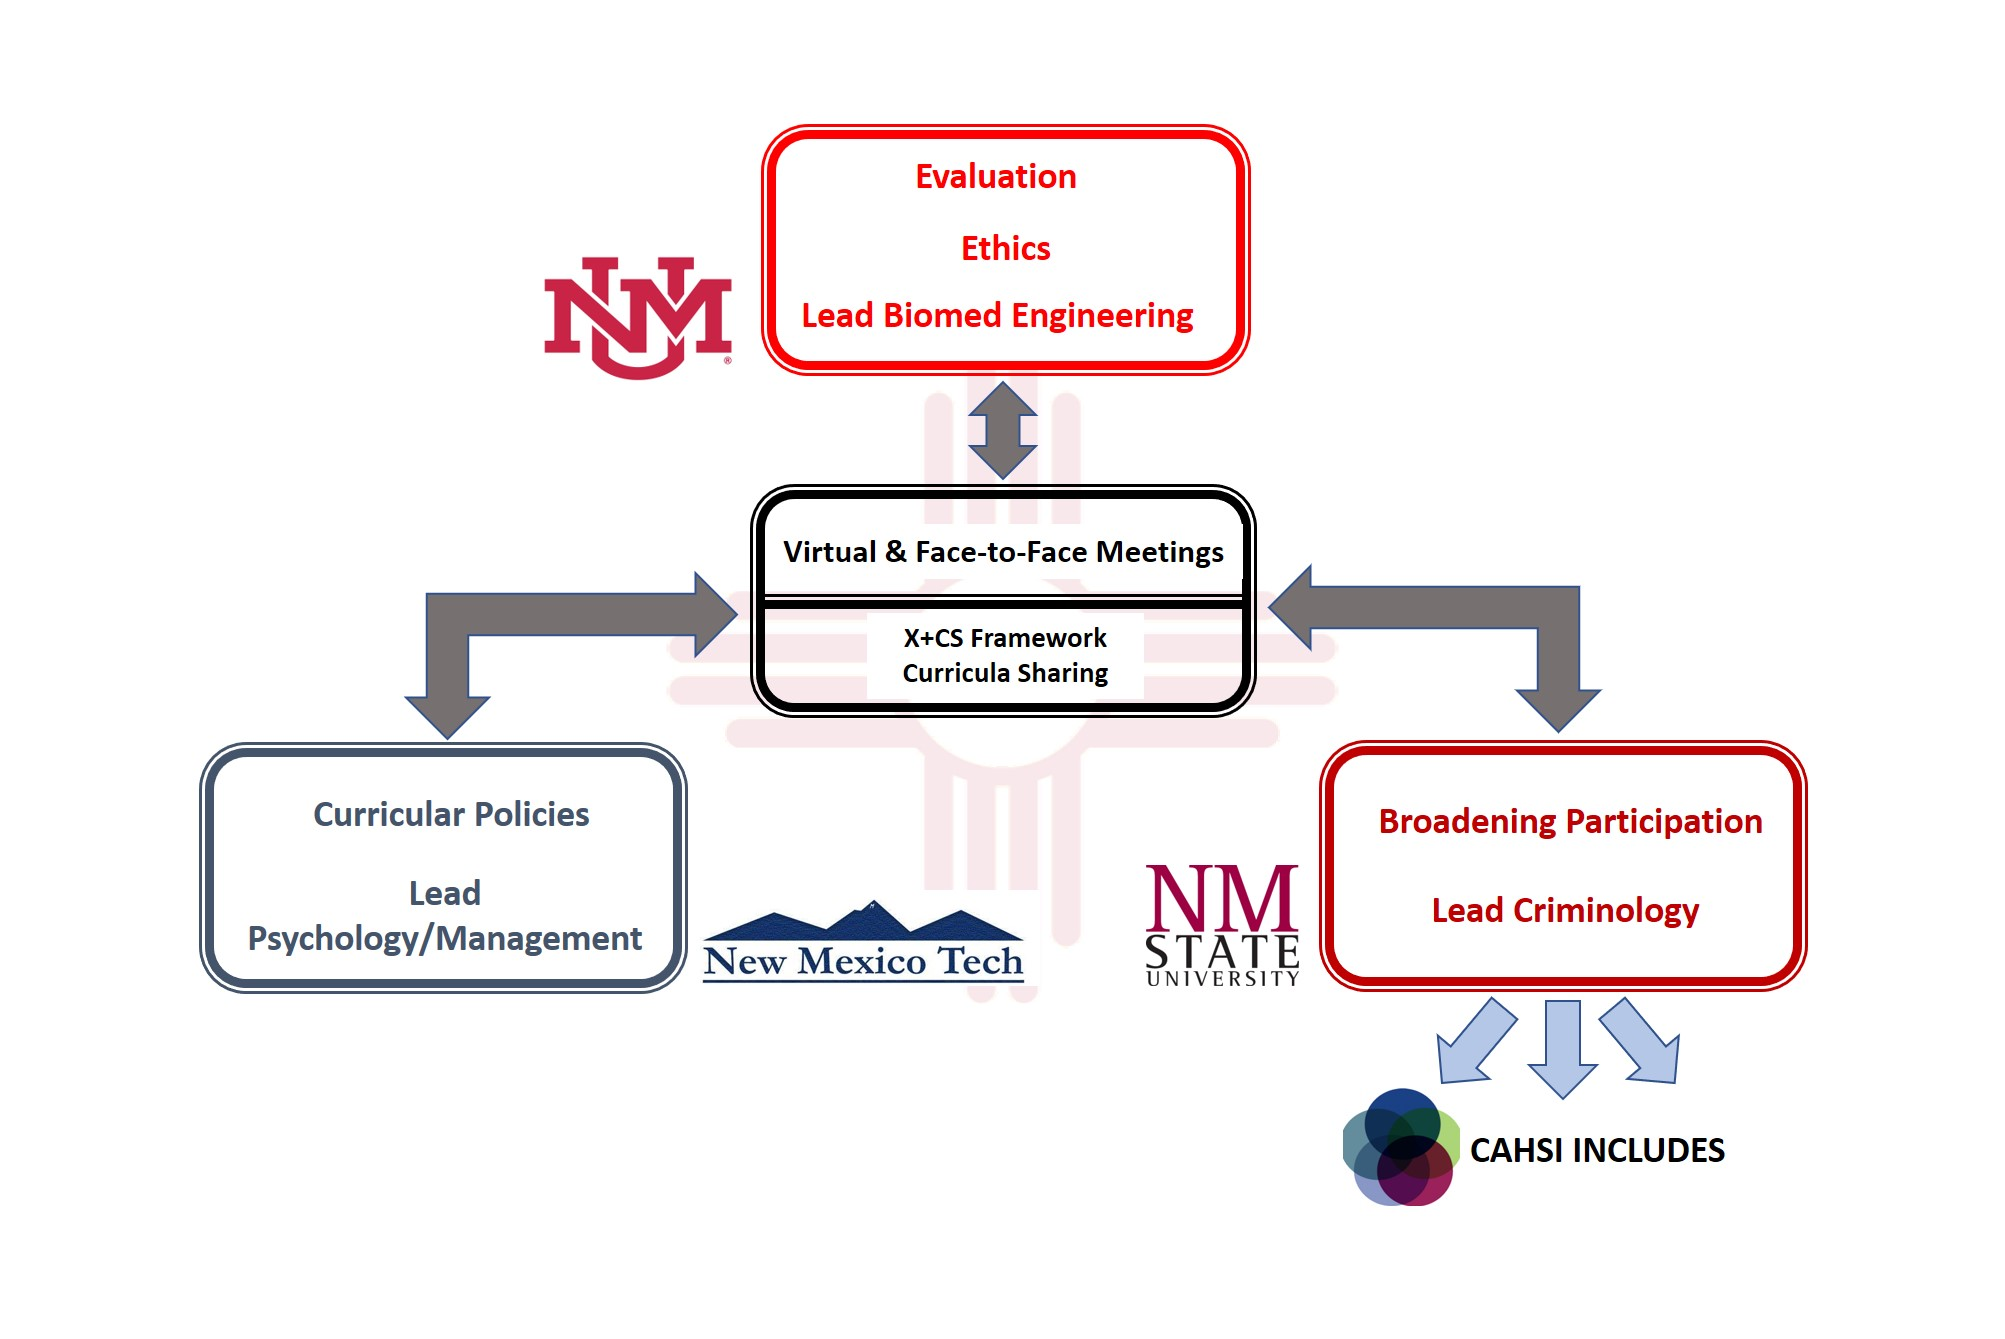
\includegraphics[width=.8\textwidth]{nic.pdf}}
\caption{Structure of the NIC}
\label{nic}
\end{figure}

 


\subsection{Existing Cross-Institution Collaborations}
The three institutions have a long history of collaborative work in the computing arena. For example, NMSU and NMT are partner in an ongoing S-STEM effort focused on promoting training of students in cybersecurity and transition of students from 2-year programs into NMSU and NMT 4-year computing degree programs (NSF Award \#1833630). The program awards scholarships to students pursuing degrees in computing disciplines and provide them with professional development opportunities, opportunities for participation in research programs, and dedicated mentoring, especially to facilitate transition of students from 2-year to 4-year programs. The partnership extends to a collection of community colleges, including community colleges with a high concentration of underrepresented students (e.g., NMSU-Grants with 31\% Native American students, Dona Ana Community College with 72.5\% Hispanic students).

UNM, NMSU and NMT participate in a state-wide collaboration, under the umbrella of the NM SMART Grid Center (Secure, Modular, Adaptive, Resilient and Transactive) to promote research and training in areas relevant to cyber-physical systems, especially in the electrical energy domain (NSF Award \#1757207). The NM SMART Grid Center is led by researchers in Computer Science and Electrical and Computer Engineering at the three institutions, with a heavy emphasis on the computational aspects of designing, controlling and operating complex cyber-physical infrastructures. NM EPSCoR provides management for the NM SMART Grid Center and has committed to convening the External Advisory Board for this project.
